\subsection{Prevention Model}
The initial evaluation is presented using the ROC curves of the normal class versus the others for selected models.
According to Figure \ref{fig:ROC_normVSrest_allmodels}, the MLP models outperformed the other models, as 
indicated by the higher AUC values.
Specifically, \textit{MLP\_Ensemble5} achieved the highest AUC value of 0.96, followed 
by \textit{MLP\_Ultra}, \textit{MLP\_Rollercoaster}, \textit{MLP\_Ensemble2}, 
and \textit{MLP\_Ensemble4}, all with an AUC of 0.95.

\begin{figure}[H]
    \centering
    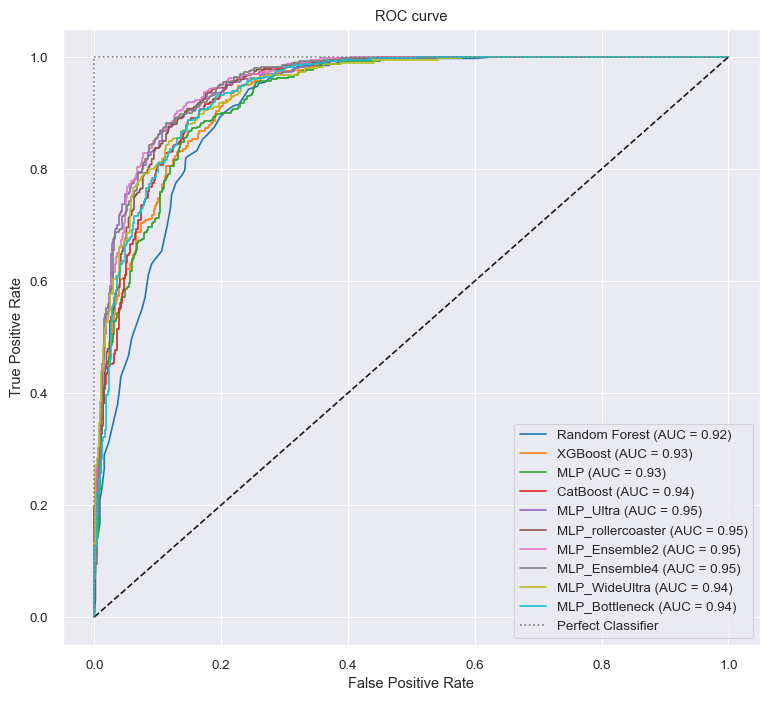
\includegraphics[width=1\columnwidth]{./images/ROC_normVSrest_allmodels.png}
    \caption{ROC curves for the normal class against the rest of the classes across all models.}
    \label{fig:ROC_normVSrest_allmodels}
\end{figure}

To further analyze model performance, we selected four significative FPR levels (1\%, 5\%, 10\%, 20\%) and 
calculated the corresponding TPR. The consolidated results are shown in 
Figure \ref{fig:normVSrest_all}.

\begin{figure*}[htpb]
    \centering
    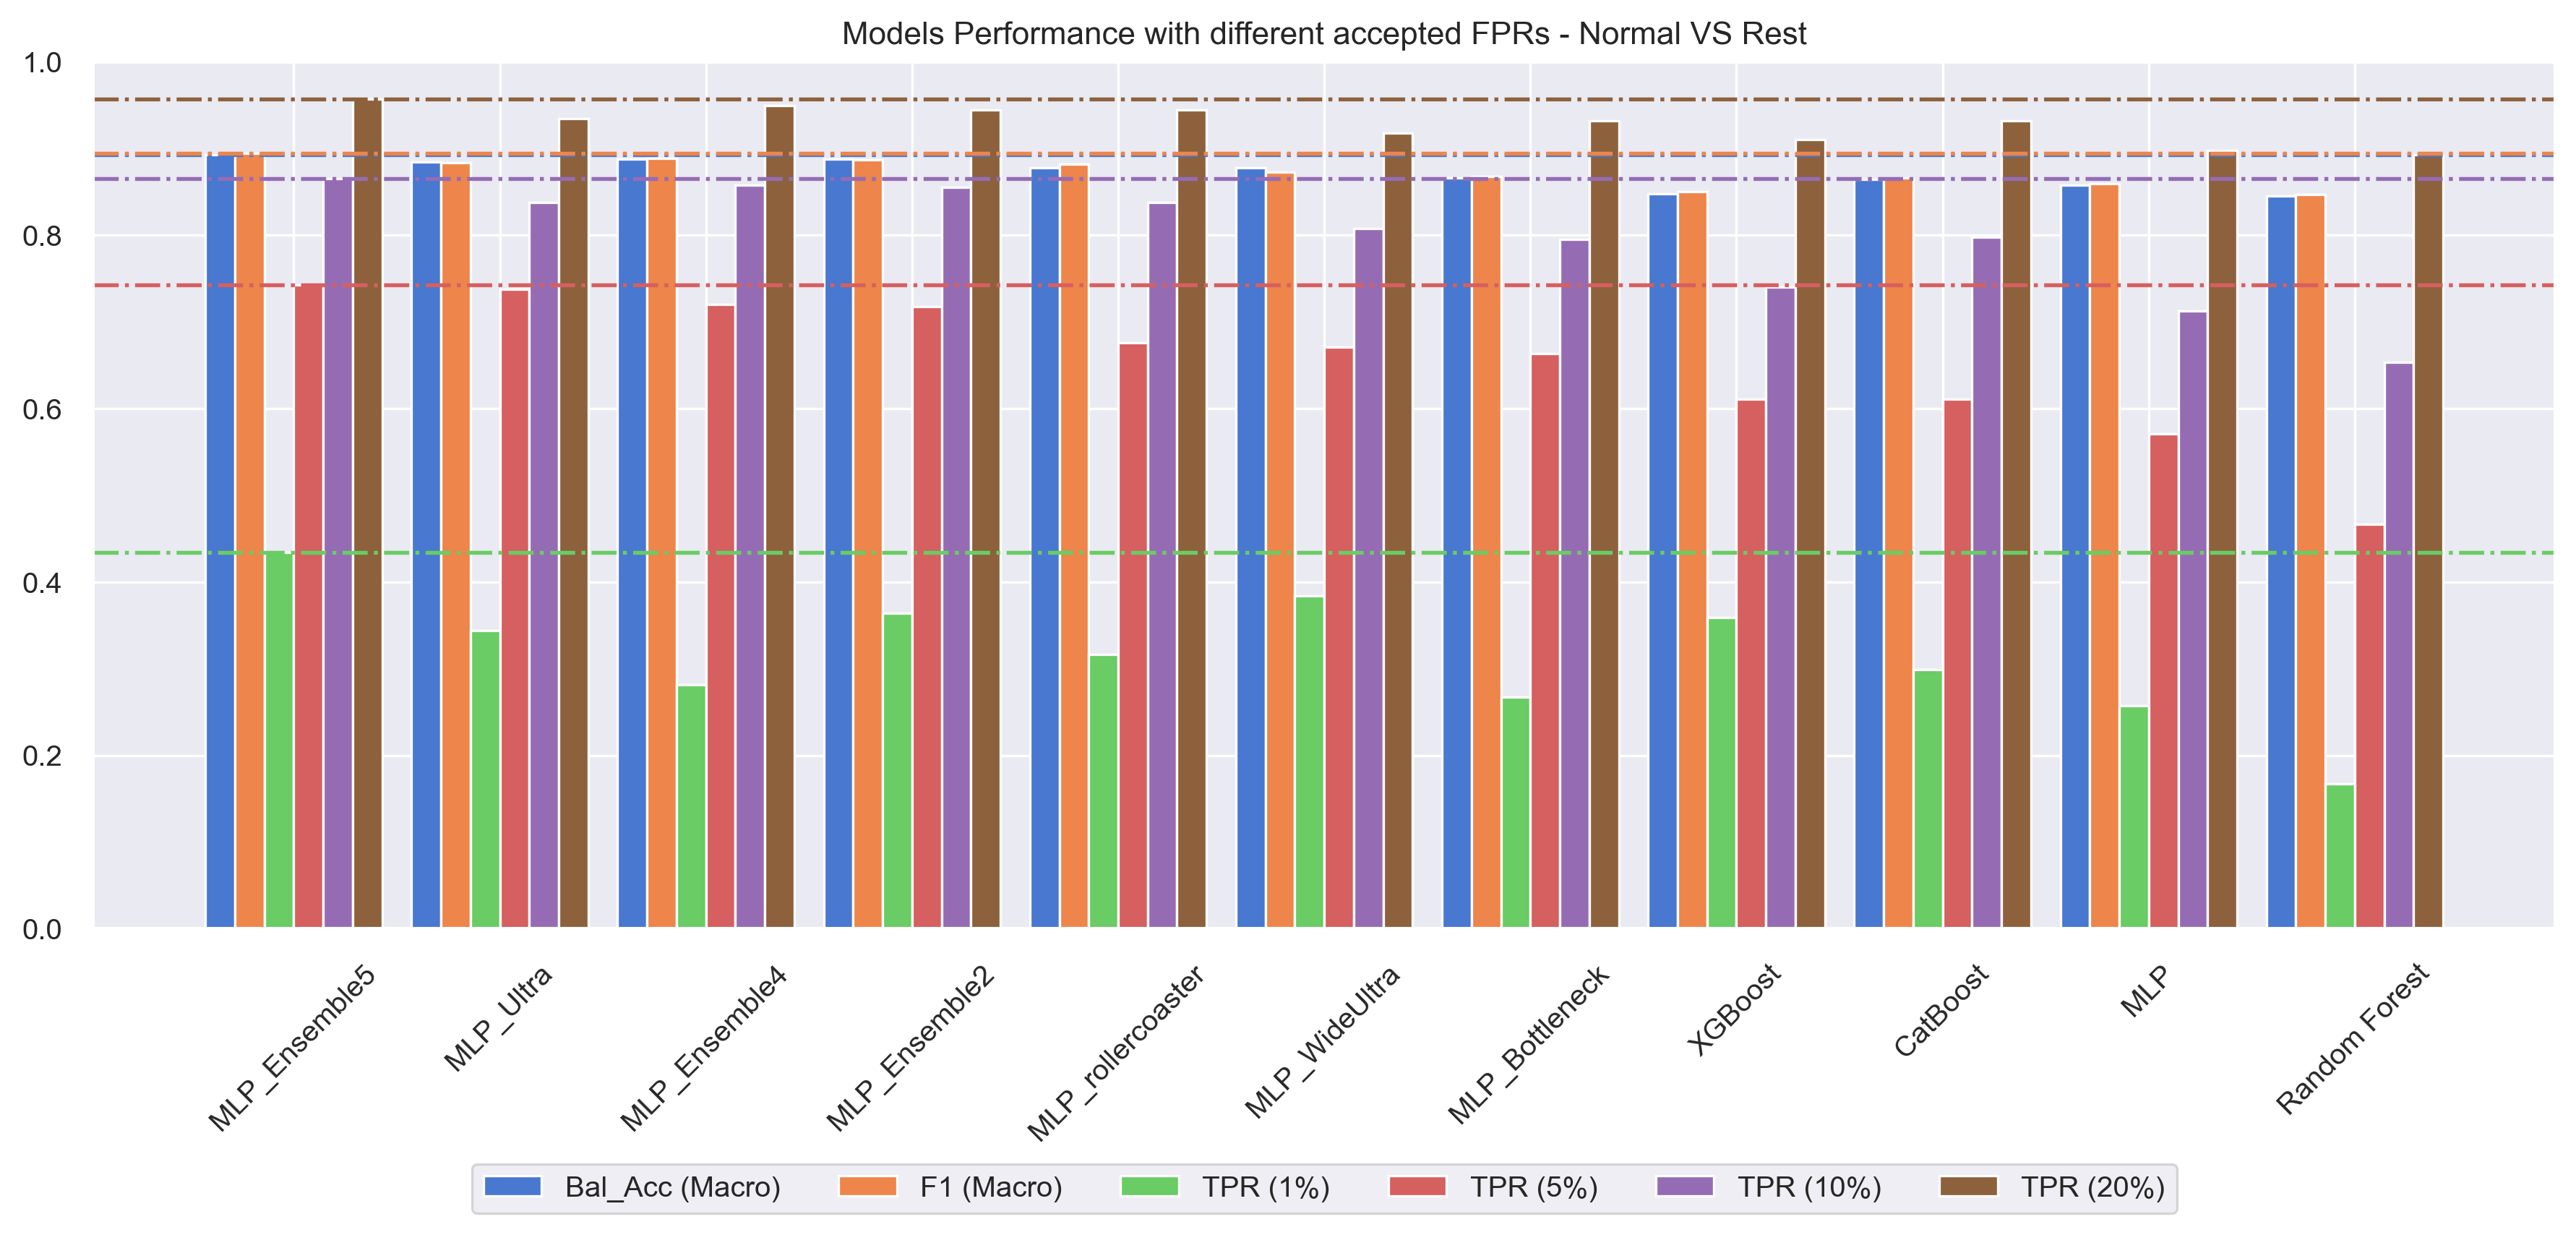
\includegraphics[width=1\textwidth]{./images/nomrVSrest_all.png}
    \caption{TPR at different FPR levels for all models.}
    \label{fig:normVSrest_all}
\end{figure*}

At each FPR level, \textit{MLP\_Ensemble5} outperformed the other models, 
achieving TPRs of 43.4\%, 74.3\%, 86.6\%, and 95.8\% at the 1\%, 5\%, 10\%, and 20\% FPR levels, 
respectively. Excluding \textit{MLP\_Ensemble5}, the best-performing model varied by 
FPR level: \textit{MLP\_WideUltra} at 1\%, \textit{MLP\_Ultra} at 5\%, \textit{MLP\_Ensemble2} at 10\%, 
and \textit{MLP\_Ensemble4} at 20\%.

These outcomes highlight the task's challenges in creating a model that performs well across all FPR 
levels and demonstrate the efficacy of a well-built ensemble model, which leverages the strengths of 
different models to achieve optimal performance.

\subsubsection{Best Model Analysis}
%confmat of the models composing it vs confmat of the ensemble

To understand the performance of the ensemble model (detailed architecture depicted in Figure \ref{fig:MLP_Ensemble5}), we compared its confusion matrix against 
the confusion matrices of the individual models that compose it
(Figure \ref{fig:confmat_ensemble_vs_individual}).

\begin{figure}[H]
    \centering
    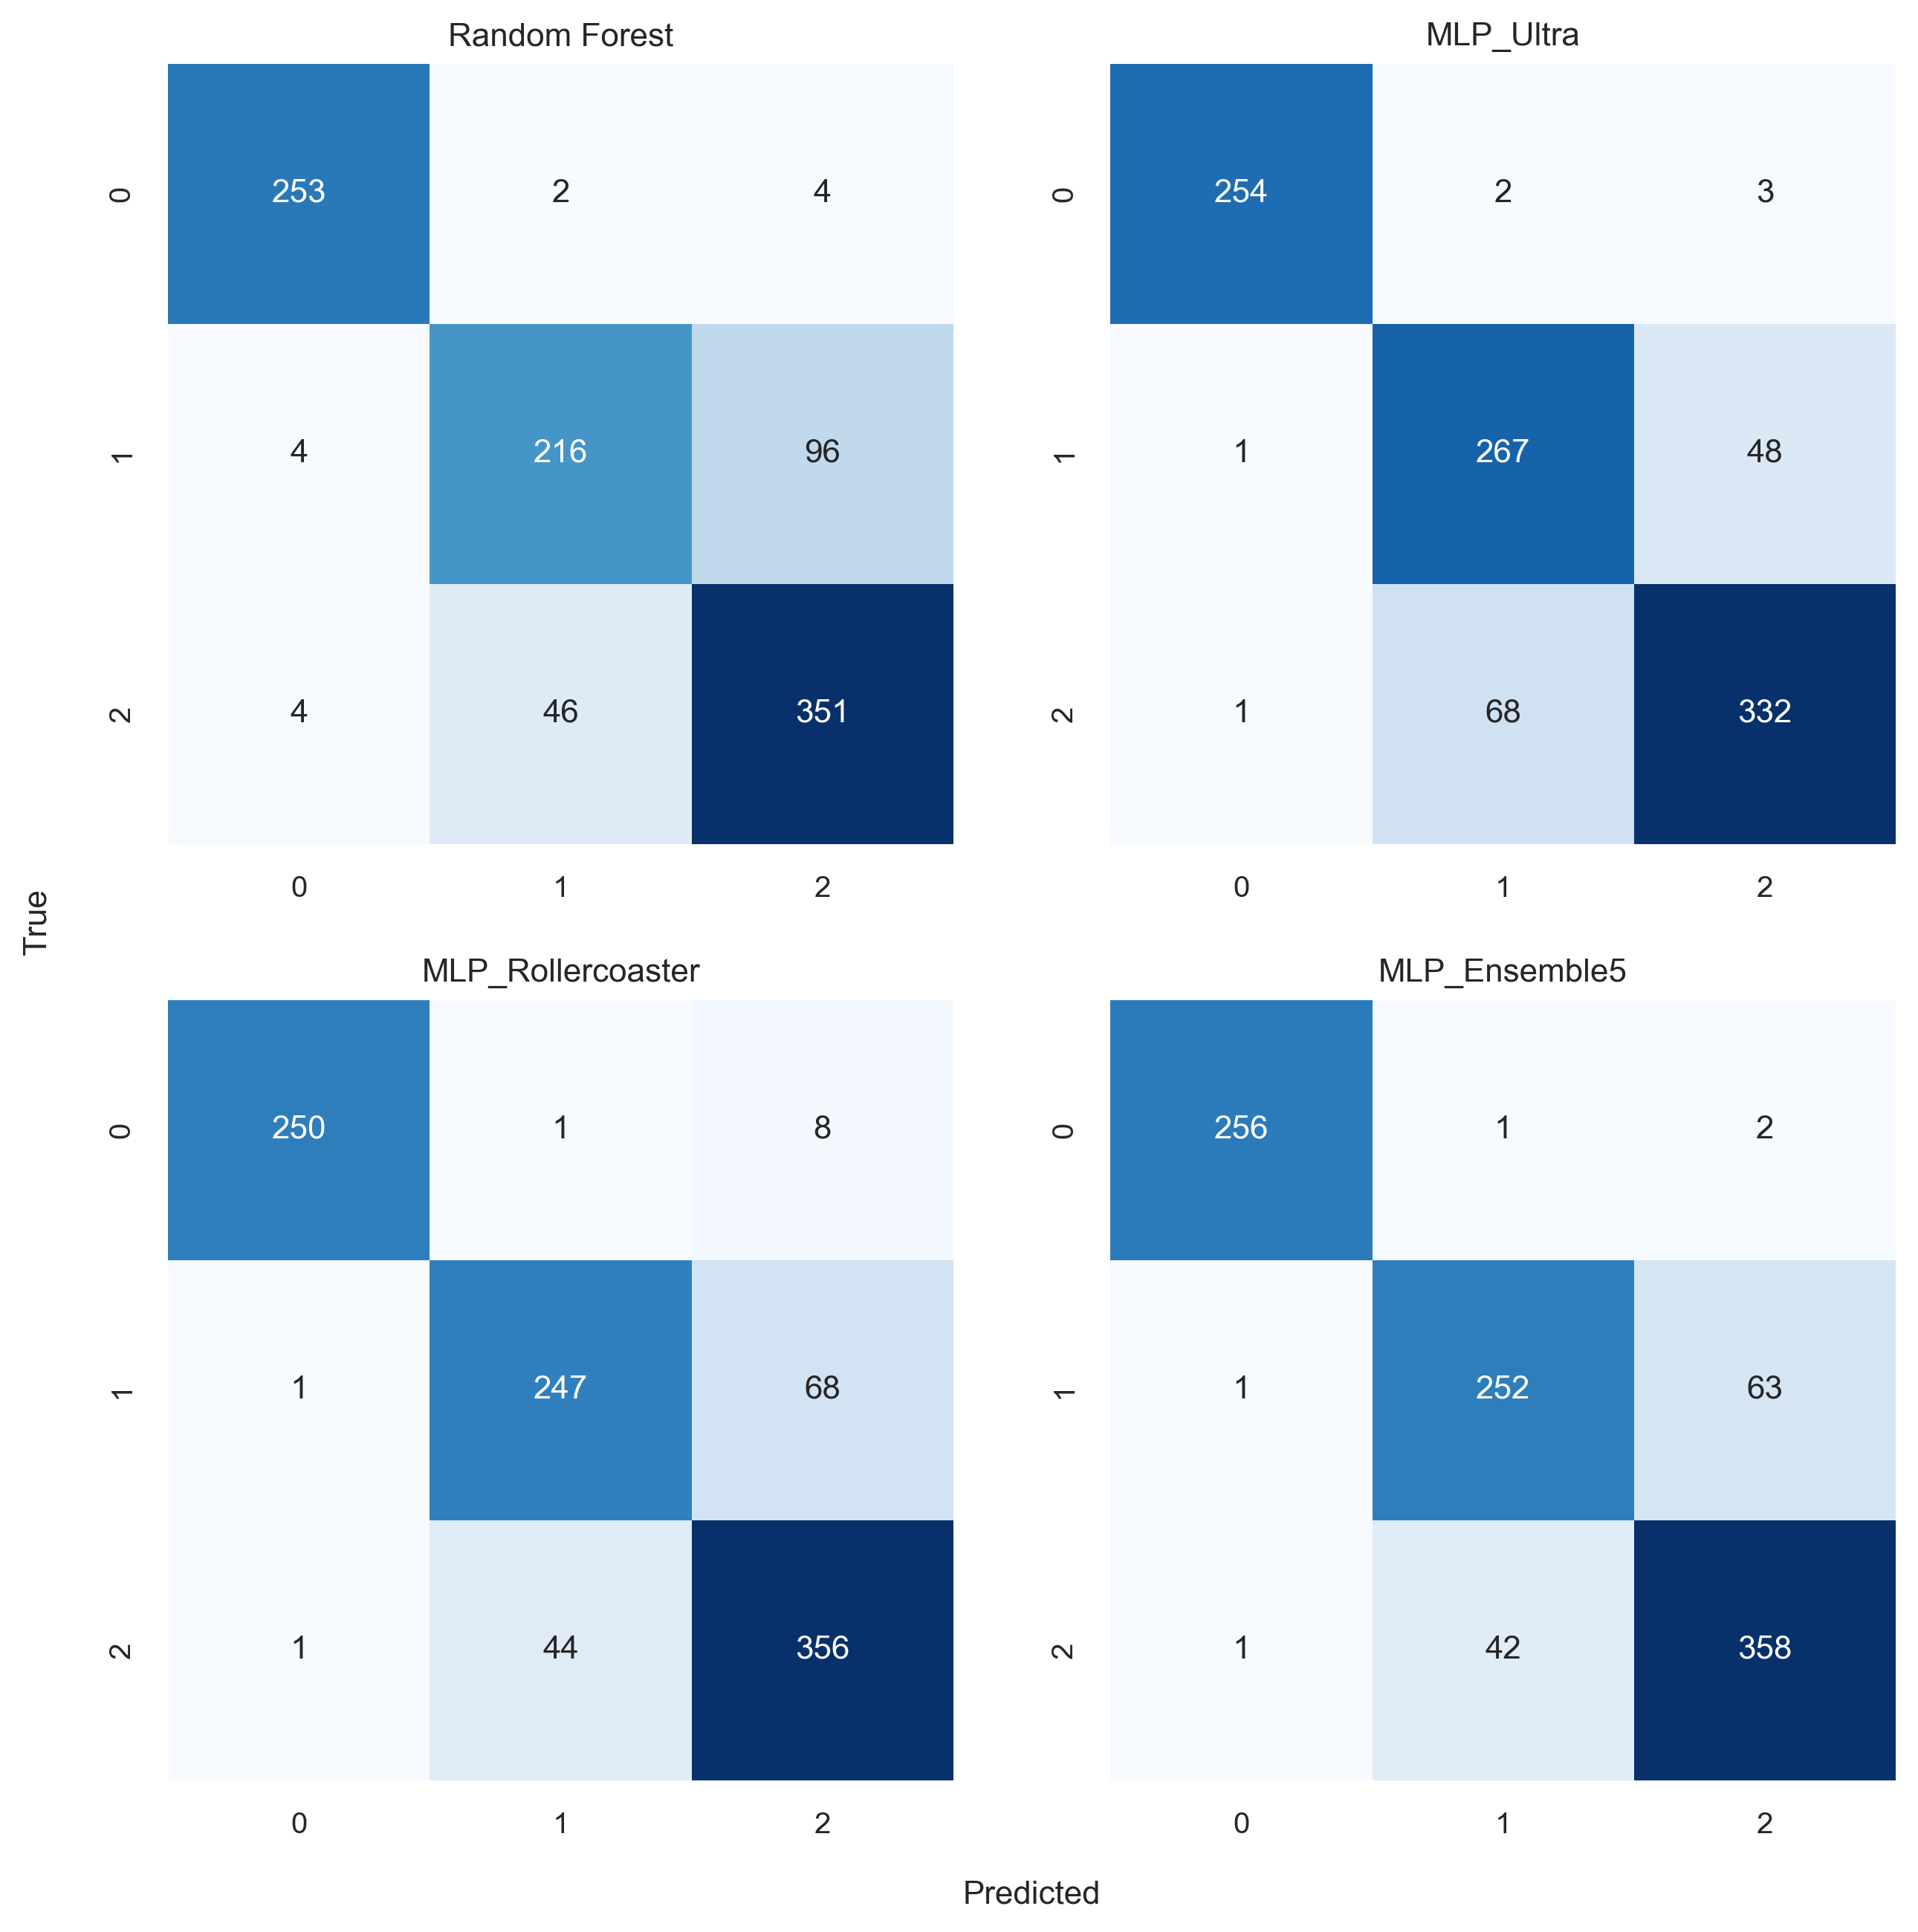
\includegraphics[width=1\columnwidth]{./images/confmat_ensemble_vs_individual.png}
    \caption{Confusion matrices of the individual models and the ensemble model.}
    \label{fig:confmat_ensemble_vs_individual}
\end{figure}

\noindent
In the confusion matrix, class 2 represents normal heartbeats, class 1 represents abnormal heartbeats, and 
class 0 represents artifacts. The Random Forest and MLP\_Ultra models exhibit complementary strengths: the 
Random Forest works better in recognizing normal samples, while the MLP\_Ultra model performs better in 
identifying abnormal samples. The ensemble model effectively combines these strengths.\\\noindent
The contribution of the MLP\_Rollercoaster model to the ensemble’s performance is less apparent but has been 
experimentally demonstrated. This may be due to its ability to correctly classify some samples that are 
misclassified by the other models.\\\noindent
Notably, the MLP\_Ultra model classifies fewer abnormal heartbeats as normal compared to the MLP\_Ensemble5 
model. However, this is because the MLP\_Ultra model simply classifies fewer samples as normal. Minimizing 
the false positive rate (FPR) for the normal class by classifying all samples as abnormal would result in a very 
low true positive rate (TPR) for the normal class. This highlights the importance of analyzing FPR and TPR together.\\\noindent
In conclusion, the ensemble model is the most effective for classifying normal heartbeats, abnormal heartbeats, 
and artifacts, achieving an optimal trade-off between FPR and TPR.